\chapter{La unión PN}

Definimos como unión $pn$ a un semiconductor al cual se le aplica en una región un dopado tipo $p$ y en otra región un dopado tipo $n$, de tal modo que $N_A \gg N_D$ en $x<0$ y $N_D \gg N_A$ en $x>0$. El estudio y caracterización de la unión $pn$ es fundamental para entender la electrónica moderna. Existen 3 situaciones en las que podemos estudiar la unión pn, que son:

\begin{itemize}
    \item \textbf{Equlibrio termodinámico}, en el que no aplicamos una diferencia de potencial $V_A$ entre la  zona $p$ y zona $n$ externa.
    \item \textbf{Polarización directa} en el que aplicamos una diferencia de potencial $V_A>0$, es decir, polarizamos $p$ respecto $n$.
    \item \textbf{Polarización inversa} en el que aplicamos una diferencia de potencial $V_A<0$, es decir, polarizamos $n$ respecto $p$.
\end{itemize} 

\section{Equilibrio termodinámico}

\subsection{Introducción}

Entendemos por \textit{equilibrio termodinámico} a la situación en la que no hay corriente externa palicada, no hay iluminación y tampoco hay gradientes de la temperatura. Además consideramos las siguientes suposiciones:

\begin{itemize}
    \item Dispositivo unidimensional.
    \item Unión metalúrgica en $x_j=0$. 
    \item Contactos óhmicos perfectos.
\end{itemize} 
Debido a la aparición de esta diferencia de dopado aparece una región alrededor de $x=0$ en el que $n$ y $p$ se difunden, esto es, $n\neq N_D$ u $p\neq N_A$, tal que $n$ y $p$ dependen de $x$. A esta región la llamamos \textbf{zona de vaciamiento}, y en ella aparece un campo eléctrico no nulo en virtud de la ecuación de Maxwell-Poisson:

\begin{equation}
    \div \Encal = \frac{\rho}{K_S \varepsilon_0}
\end{equation}
siendo $\rho=-qn(x)+qp(x)$, y como $V(x)=-\int \Ecal \D x$, también aparece un potencial no cpnstate (siempre en la zona de vaciamiento). Como sabemos, existe una relación entre $V$ y las energías $E_i,E_v$ y $E_c$. 

\begin{equation*}
    q \parciales{V}{x} = - \parciales{E_i}{x}
\end{equation*}
y como $E_F$ es contante en el equlibrio. Definimos como \textbf{unión pn escalon} a aquella unión $pn$ en la que con regiones $p$ y $n$ dopados uniformemente, con un salto abrupto en $x=0$.. Es el caso más sencillo y más usado. El esquema de bandas es:


Cabe destacar que la caracterización de cualquier unión $pn$ (sea escalón, gradual...) es muy similar, presentando esquemas de bandas similares, solo cambiando la forma en la región de vaciamiento.


\subsection{Caracterización de la unión pn escalón}
Caracterizar la unión $pn$ es equivalente a conocer la densidad de carga, el campo eléctrico y el potencial a lo largo del dispositivo, a sí como la anchura de la región de vaciamiento. Muchos de estos valores están relacionados entre sí, y todos ellos dependen de el nivel de dopado $(N_D,N_A)$ del material ($E_g,n_i$) y de la temperatura ($T$). La mayor parte de estos los calcularemos a partir de aproximaciones. Lo que si podemos calcular sin hacer (casi) ninguna aproximación es $V_{bi}$. Hay dos maneras de calcular $V_{bi}$, a saber, por energías y por corrientes. El cálculo por energías es el más sencillo, y por el que nosotros optamos. Se define $V_{bi}$ como:
\begin{equation}
    V_{bi}= 
\end{equation}

\subsection{Caracterización de la unión pn gradual}

%%%%%%%%%%%%%%%%%%%%%%%%%%%%%%%%%%%%%%%%%%%%%%%%%%%%%%%%%%%%%%%%%%%%%%%
%%%%%%%%%%%%%%%%%%%%%%%%%%%%%%%%%%%%%%%%%%%%%%%%%%%%%%%%%%%%%%%%%%%%%%%
%%%%%%%%%%%%%%%%%%%%%%%%%%%%%%%%%%%%%%%%%%%%%%%%%%%%%%%%%%%%%%%%%%%%%%%
%%%%%%%%%%%%%%%%% UNION PN BAJO POLARIZACIONES %%%%%%%%%%%%%%%%%%%%%%%%
%%%%%%%%%%%%%%%%%%%%%%%%%%%%%%%%%%%%%%%%%%%%%%%%%%%%%%%%%%%%%%%%%%%%%%%
%%%%%%%%%%%%%%%%%%%%%%%%%%%%%%%%%%%%%%%%%%%%%%%%%%%%%%%%%%%%%%%%%%%%%%%
%%%%%%%%%%%%%%%%%%%%%%%%%%%%%%%%%%%%%%%%%%%%%%%%%%%%%%%%%%%%%%%%%%%%%%%

\section{Union pn bajo polarizaciones}

En una situación de equilibrio la densidad de electrones $n$ en la zona $n$ de la unión será mucho mayor que en la zona $p$. Esta diferencia de densidades provocará la aparición de una corriente de difusión de la región $n$ a la región $p$. Sin emargo, la existencia de una diferencia de potencial entre la zona $n$ y la zona $p$ genera un campo eléctrico contrario a la corriente de difusión.


%%%%%%%%%%%%%%%%%%%%%%%%%%%%%%%%%%%%%%%%%%%%%%%%%%%%%%%%%%%%%%%%%%%%%%%
%%%%%%%%%%%%%%%%%%%%%%%%%%%%%%%%%%%%%%%%%%%%%%%%%%%%%%%%%%%%%%%%%%%%%%%
%%%%%%%%%%%%%%%%%%%%%%%%%%%%%%%%%%%%%%%%%%%%%%%%%%%%%%%%%%%%%%%%%%%%%%%
%%%%%%%%%%%%%% CARACTERISTICAS IV DE LA UNION PN %%%%%%%%%%%%%%%%%%%%%%
%%%%%%%%%%%%%%%%%%%%%%%%%%%%%%%%%%%%%%%%%%%%%%%%%%%%%%%%%%%%%%%%%%%%%%%
%%%%%%%%%%%%%%%%%%%%%%%%%%%%%%%%%%%%%%%%%%%%%%%%%%%%%%%%%%%%%%%%%%%%%%%
%%%%%%%%%%%%%%%%%%%%%%%%%%%%%%%%%%%%%%%%%%%%%%%%%%%%%%%%%%%%%%%%%%%%%%%



%%%%%%%%%%%%%%%%%%%%%%%%%%%%%%%%%%%%%%%%%%%%%%%%%%%%%%%%%%%%%%%%%%%%%%%
%%%%%%%%%%%%%%%%%%%%%%%%%%%%%%%%%%%%%%%%%%%%%%%%%%%%%%%%%%%%%%%%%%%%%%%
%%%%%%%%%%%%%%%%%%%%%%%%%%%%%%%%%%%%%%%%%%%%%%%%%%%%%%%%%%%%%%%%%%%%%%%
%%%%%%%%%%%%%%%%%%%%%%%%  EJERCICIOS %%%%%%%%%%%%%%%%%%%%%%%%%%%%%%%%%%
%%%%%%%%%%%%%%%%%%%%%%%%%%%%%%%%%%%%%%%%%%%%%%%%%%%%%%%%%%%%%%%%%%%%%%%
%%%%%%%%%%%%%%%%%%%%%%%%%%%%%%%%%%%%%%%%%%%%%%%%%%%%%%%%%%%%%%%%%%%%%%%
%%%%%%%%%%%%%%%%%%%%%%%%%%%%%%%%%%%%%%%%%%%%%%%%%%%%%%%%%%%%%%%%%%%%%%%

\newpage

\section{Ejercicios}



\subsection{Ejercicio 1}


Ejercicio 1


\rule{\textwidth}{0.1pt} \\[2pt]

Vamos a calcular las masas efectivas en función de las movilidades y las vidas medias:

\begin{equation}
    \mu_n = D_n \frac{q}{kT} = \frac{q}{kT} \tau_n v^2_{th} = \frac{q}{kT} \tau_n \frac{3kT}{m_n^*} = \frac{3q\tau_n}{m_n^*}
\end{equation}
Entonces:
\begin{equation}
    m_n^* = \frac{3q\tau_n}{\mu_n} \qquad m_p^* = \frac{3q\tau_p}{\mu_p^*}
\end{equation}
Usando estas ecuacioens obtenemos:

\begin{equation}
    m_p^* = 3.88 \cdot 10^6 \ m_e \tquad m_n^* = 11.5 \cdot 10^6 \ m_e
\end{equation}
Francamente no se que puede estar mal, pero usaremos las masas típicas $m_p^* = 0.81m_e$ y $m_n=1.18 m_e$. 
\begin{enumerate}[label=\alph*)]
    \item Tenemos que calcular la anchura de todas las regiones del dispositivo y las bandas de energía (banda de conducción, banda de valencia, nivel de Fermi y nivel de Fermi intrínseco). También tenemos que calcular las distancias relativas entre los niveles (lo cual es obvio dado lo anterior). 
    
    Primero tenemos que calcular las distancias, lo cual es simplemente aplicar las fórmulas para la situación de equilibrio
    \begin{equation}
        x_p = \ccorchetes{\frac{2K_S\varepsilon_0}{q} \frac{N_D}{N_A(N_A+N_D)}  V_{bi}}   \qquad 
        x_n = \ccorchetes{\frac{2K_S\varepsilon_0}{q} \frac{N_A}{N_D(N_A+N_D)}  V_{bi}}
    \end{equation}
    Así pues, los valores numéricos son: 

    \begin{equation}
        x_p = 5.000\cdot 10^{-5}  \ [\cm] \qquad x_n =1.000\cdot 10^{-4}  \ [\cm] \qquad W = x_n + x_p = 1.5 \cdot 10^{-4} \ [\cm ]
    \end{equation}
    Y luego tenemos que calcular los valores de todas y cada una de las bandas. Para conocer las banda, teniendo en cuenta que $E_F=0 \ [\eV]$  \textit{a lo largo de todo el dispositivo pn}. Por el resto simplemente aplicar las ecuaciones de la sección 2, tal que en la zona $p$ los valores son los que típicamente esperaríamos para un semiconductor $N_A$, mientras que en la zona $n$ será los que esperaríamos en un conductor $N_A$ menos $V_{bi}$. En la \textit{zona de vaciamiento} los valores de las bandas simplemente valdrán su valor en $p$ menos el valor $V(x)$:
    \begin{equation*}
        V_{bi} = \frac{kT}{q} \ln \parentesis{\frac{N_AN_D}{n_i^2}} = 0.580 \ [\unit{V}]
    \end{equation*}
    \begin{equation*}
        V(x) = \left\lbrace \begin{array}{ll}
            - \frac{qN_A}{2K_S\varepsilon_0} \parentesis{x_p + x}^2  & \ - x_p \leq x \leq 0 \\
            - \frac{qN_D}{2K_S\varepsilon_0} \parentesis{x_n - x}^2 + V_{bi}  & \ 0 \leq x \leq x_n \\
        \end{array} \right.
    \end{equation*}
    Por el resto de situaciones, tenemos que en la zona $p$ las ecuaciones son:
    \begin{equation*}
        E_i = - kT \ln \parentesis{\frac{n}{n_i}} = kT \ln \parentesis{\frac{N_A}{n_i}} \qquad E_c  = E_i  + kT \ln \parentesis{\frac{N_c}{n_i} } \qquad E_v  =E_c-E_g
    \end{equation*}
    tal que 
    \begin{equation*}
        E_g = 1.12 \ [\eV] \qquad N_C = 2 \parentesis{\frac{m_n^* kT}{2\pi \hbar^2}}^{3/2}  = 3.21 \cdot 10^{19} \ [\cm^{-3}] \end{equation*}
    \begin{equation*}    
       N_V = 2 \parentesis{\frac{m_p^* kT}{2\pi \hbar^2}}^{3/2} = 1.83 \cdot 10^{19} \ [\cm^{-3}] 
    \end{equation*}
    \begin{equation*}
        n_i = \sqrt{N_CN_V} e^{-E_g/kT} = 9.49 \cdot 10^9 \ [\cm^{-3}]
    \end{equation*}
    Así pues obtenemos los siguientes resultados numéricos: 
    \begin{center}
        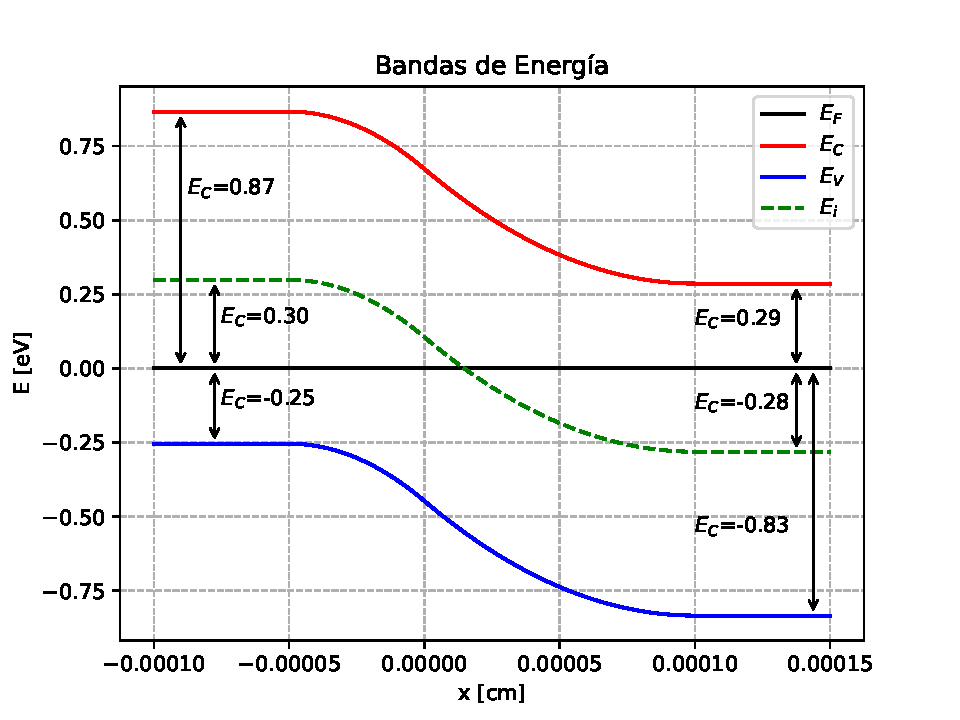
\includegraphics[width=0.6\linewidth]{Cuerpo/Ch_03/03_01_Bandas.pdf}
    \end{center}
    \item Si polarizamos la zona N con 0.2 voltios ($V_A=-0.2$V) estamos en el régimen de polarización inversa. El calculo de los anteriores valores es exáctamente igual solo que ahora tenemos que $V_{bi}\rightarrow V_{bi}-V_A$. Así pues:
    \begin{equation}
        x_p = 5.79867 \cdot 10^{-5}  \ [\cm ] \tquad
        x_n = 1.15973 \cdot 10^{-4}  \ [\cm ]
    \end{equation}xp=[cm]
    \begin{center}
        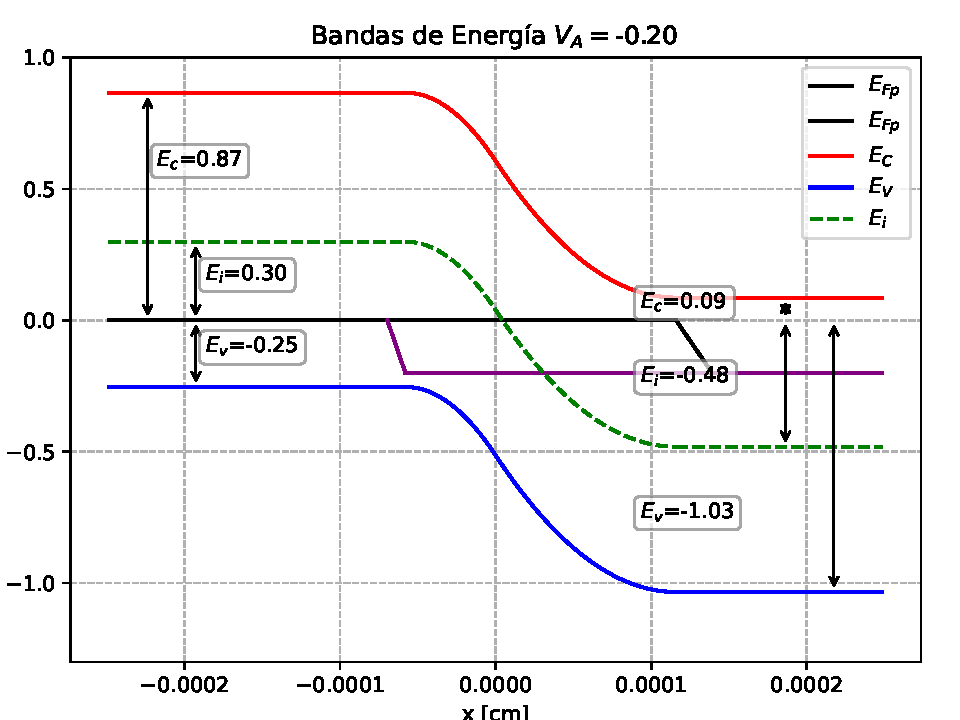
\includegraphics[width=0.6\linewidth]{Cuerpo/Ch_03/03_02_Bandas.pdf}
    \end{center}

    \item Si polarizamos la zona P con 0.2 voltios ($V_A=0.2$V) estamos en el régimen de polarización directa. El calculo de los anteriores valores es exáctamente igual solo que ahora tenemos que $V_{bi}\rightarrow V_{bi}-V_A$. Así pues:
    \begin{equation}
        x_n =8.09502 \cdot 10^{-5}  \ [\cm ] \tquad x_p = 4.04751 \cdot 10^{-5}  \ [\cm ]
    \end{equation}
    \begin{center}
        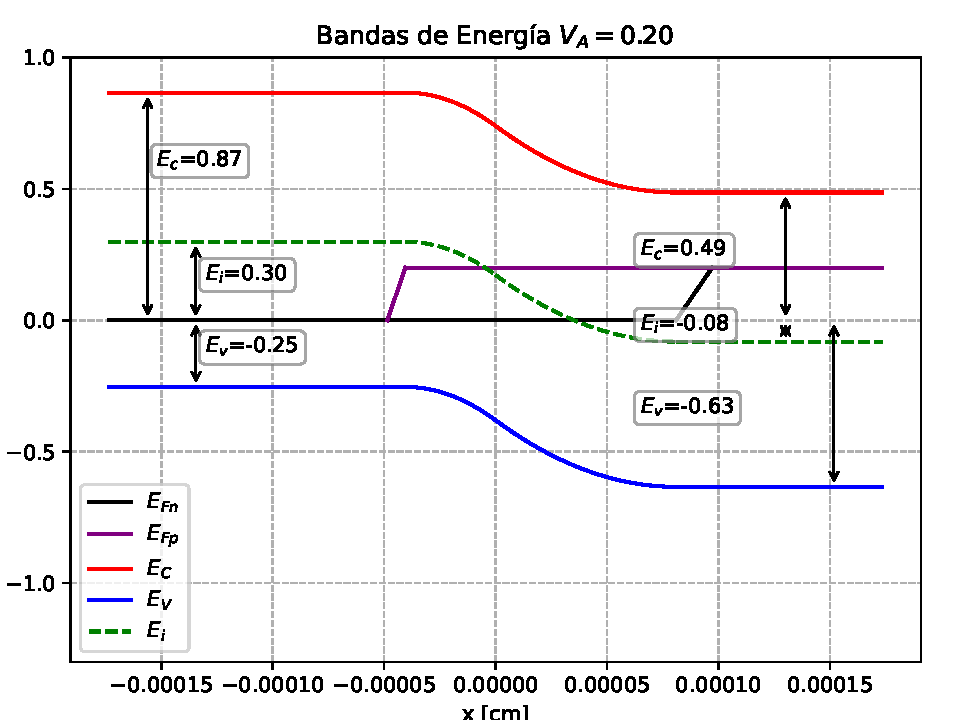
\includegraphics[width=0.6\linewidth]{Cuerpo/Ch_03/03_03_Bandas.pdf}
    \end{center}
    Ahora nos piden calcular el campo eléctrico, la densidad de carga y el voltaje a lo largo del dispositivo, así como las corrientes a lo largo del mismo. Para calcular el campo eléctrico tenemos que usar la típica fórmula:

    \begin{equation}
        \Ecal = - \derivadas{V}{x} = \frac{1}{q} \derivadas{E_i}{x}
    \end{equation}
    Así por lo tanto tenemos que: 

    \begin{equation*}
        \Ecal(x) = \left\lbrace \begin{array}{ll}
             \frac{qN_A}{K_S\varepsilon_0} \parentesis{x_p - x}  & \ - x_p \leq x \leq 0 \\
            - \frac{qN_D}{K_S\varepsilon_0} \parentesis{x_n - x} & \ 0 \leq x \leq x_n \\
        \end{array} \right.
    \end{equation*}
    siendo 0 en el resto de puntos del dispositvo. El volaje se calcula teniendo en cuenta la anterior ecuación (considerando que el cero del potencial está en la zona $p$) on la ecuación que hemos usado previamente (a). Solo falta calcular la densidad de carga, que se hace usando, por ejemplo, la ecuación de Maxwell

    \begin{equation}
        \nabla \cdot E = \frac{\rho}{K_S \varepsilon_0} 
    \end{equation}
    de tal modo que:

    \begin{equation}
        \rho (x) = \left\lbrace \begin{array}{ll}
            - q N_A   & \ - x_p \leq x \leq 0 \\
            q N_D \parentesis{x_n - x} & \ 0 \leq x \leq x_n \\
        \end{array} \right.
    \end{equation}
    Lo cual es en realidad trivial o directo, ya que procede de las hipótesis de vaciamiento que usamos para deducir todas las ecuaciones (en las condiciones que exigimos para la verificación de todas estas ecuaciones incluye que $n_n,p_p\ll N_D,N_A$) de tal modo que la ecuación de la carga es la primera condición, no la última. En cualquier caso, hacemos las representaciones gráficas:   
    \begin{center}
        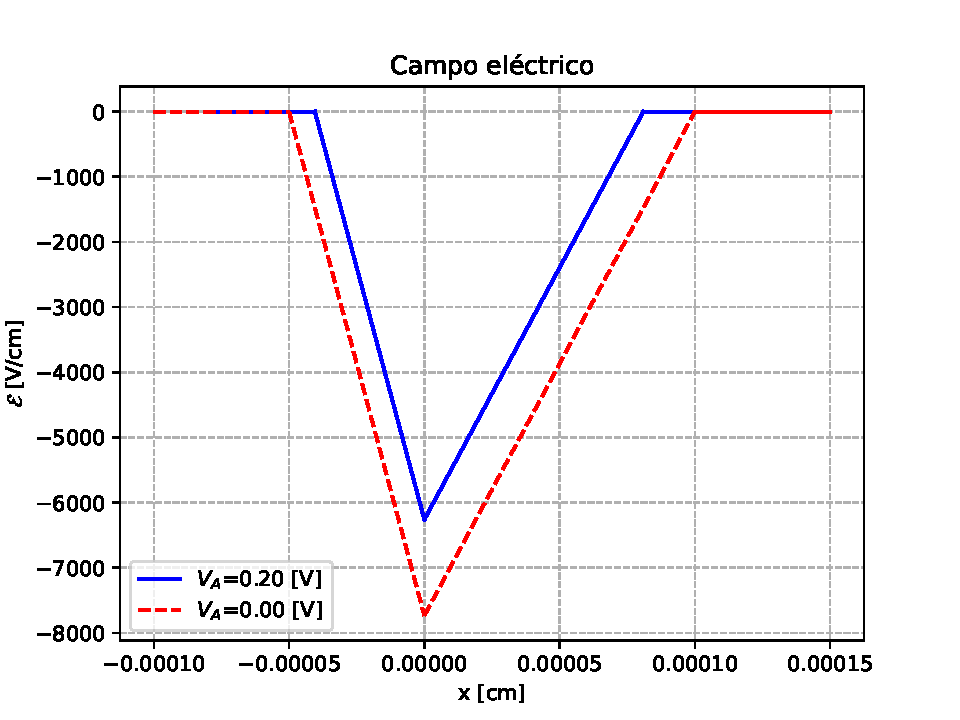
\includegraphics[width=0.6\linewidth]{Cuerpo/Ch_03/03_04_E.pdf}
    \end{center}   
    \begin{center}
        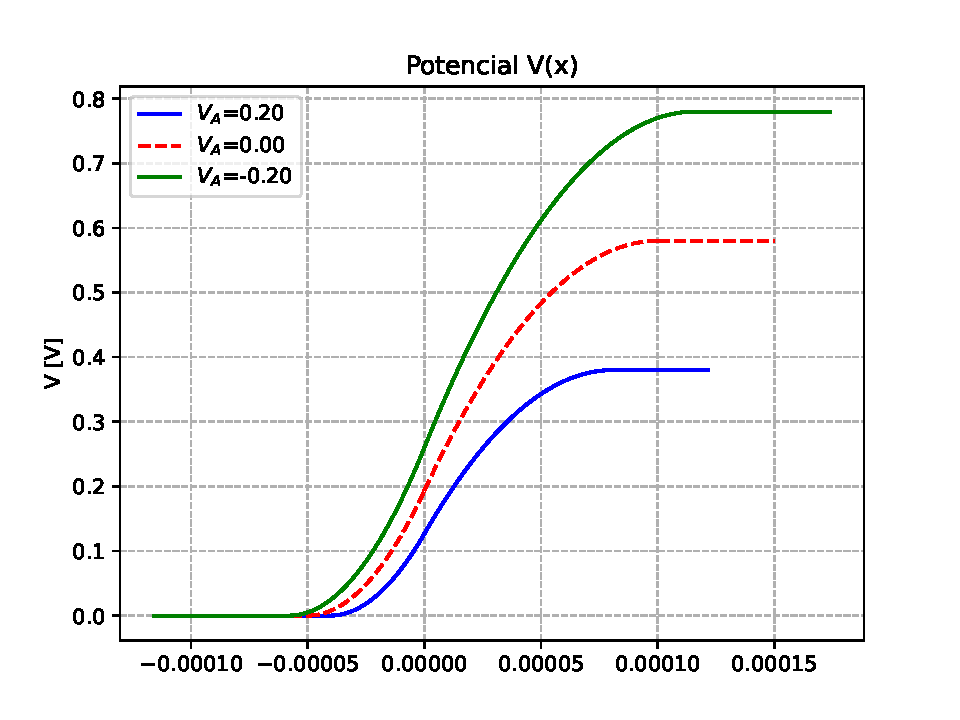
\includegraphics[width=0.6\linewidth]{Cuerpo/Ch_03/03_05_V.pdf}
    \end{center}   
    \begin{center}
        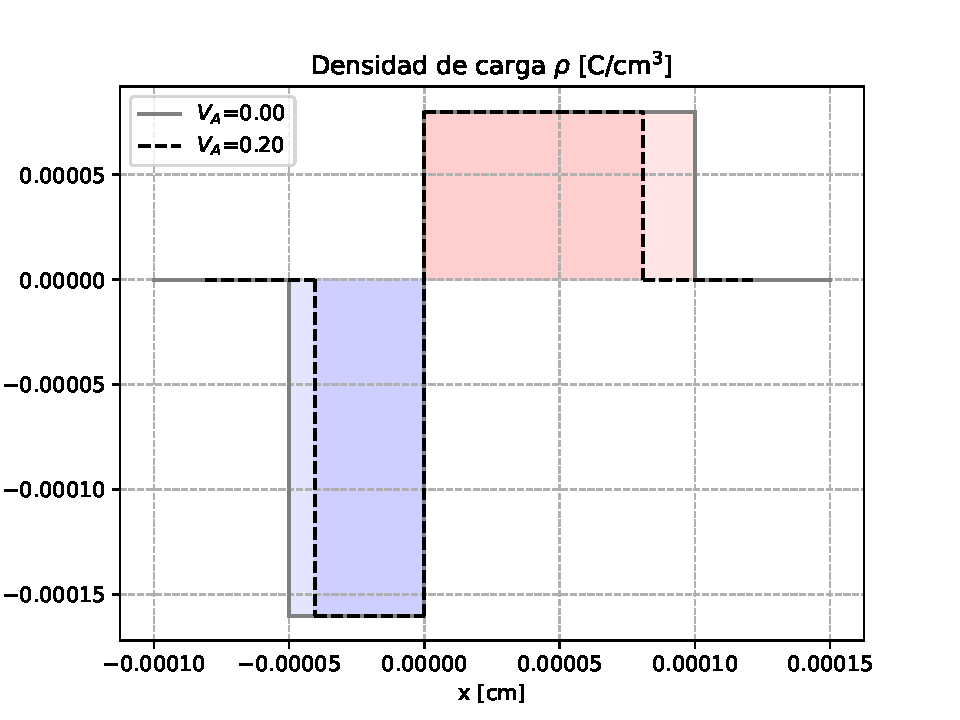
\includegraphics[width=0.6\linewidth]{Cuerpo/Ch_03/03_06_rho.pdf}
    \end{center}   
    Ahora tenemos que calcular las corrientes a lo largo del dispostivo. Las corrientes 
\end{enumerate}    

\rule{\textwidth}{0.1pt} \\[2pt]

\subsection{Ejercicios 2}

Partimos de una unión escalón NP realizada con un cristal semicondcutor de germanio ($E_G = 0.66 \ \eV$, $m_e^*=0.5$, $m_h^* = 0.37$) con $N_D=10^{16} \ \cm^{-3}$ y $N_A = 10^{15} \ \cm^{-3}$, en cada zona siendo la longitud de la zona $N$ de 0.003 cm y la de la zona P de 0.002 cm y el área de $10^{-2} \ \cm^2$. La permitividad para el germanio es de $1.4337 \times 10^{-12}$ F/cm, y el $n_i=2.0 \times 10^{13}$ cm$^{-3}$, las movilidades de electrones y huecos son $3900$ cm$^2$/(V$\cdot$s) y $1900$ cm$^2$/(V$\cdot$s) respectivamente y $\tau_n=\tau_p=10^{-6}$ s.


\rule{\textwidth}{0.1pt} \\[2pt]
